\section{Experiment Pipeline}
\label{sec:methods/section_c}

Once we selected the parameters for YOLOv3 and SORT, we will run the tracking experiment to assess tracking accuracy. The experiment will involve running the object detector and tracker on the uncompressed and compressed video sequences. For the case of compressed sequences, we apply HEVC video compression (HM16.20) at different quantization parameter (QP) and motion search range (MSR) values. Table \ref{tab:qp_msr_range} shows the range of QP and MSR chosen for the experiment.
\begin{table}[]
    \centering
    \begin{tabular}{|c|c|}
        \hline
        HEVC parameter & Range of values \\
        \hline
        \hline
        QP & [18, 22, 26, 30, 34, 38, 42, 46] \\
        \hline
        MSR & [8, 16, 32, 64] \\
        \hline
    \end{tabular}
    \caption[Selected QP and MSR range for the experiment]
    {Selected QP and MSR range for the experiment.}
    \label{tab:qp_msr_range}
\end{table}
For the case of uncompressed sequences, we do not apply HEVC compression but run the object detector and tracker directly on the raw sequences. The uncompressed sequences from Table \ref{tab:seq_list} were used, but we excluded the training sequence PartyScene since we have used this sequence to tune the parameters of the detector and tracker. Therefore, there are a total of 12 sequences in the experiments. Figure \ref{fig:experiment_pipeline} shows the pipeline for the experiment, and each step is explained as follows.

% \begin{myfont}
% \centering
% QP = [18, 22, 26, 30, 34, 38, 42, 46], MSR = [8, 16, 32, 64]
% \end{myfont}


\begin{enumerate}
    \item \textbf{HEVC Encoding}: The experiment starts with applying HEVC encoding to the uncompressed sequences and generating the compressed bitstreams. Low Delay Encoding is used for encoding. Encoding is the process that took the most amount of time in the entire pipeline, so we encoded all the possible combinations of QP and MSR and saved all the compressed bitstreams before applying the decoder.
    \item \textbf{HEVC Decoding}: After obtaining all the compressed bitstreams, we apply the HEVC decoder to the bitstreams and output the decoded sequences in the YUV420 format.
    \item \textbf{YUV420 to RGB24 color conversion}: Since the YOLOv3 object detector accepts input images in the RGB24 format, we convert the decoded sequences from YUV420 to RGB24 format and save frames in PNG files.
    \item \textbf{Running YOLOv3 and SORT}: Once the decoded sequence are stored in RGB24, we run the object detector and tracker to obtain the tracking results in MOT benchmark format. 
    \item \textbf{MOT metrics evaluation}: To assess the tracking performance, we input both the tracking results and ground truth, and the software \cite{heindl_cheindpy-motmetrics_2021} will generate the tracking performance results.
\end{enumerate}
We ran YOLOv3 and SORT to detect and track each class ID shown in Table \ref{tab:seq_list} as single-class tracking, and also detect and track the "all" object classes. In other words, we took measurements from single-class object tracking and multi-class multiple objects tracking.
\begin{figure}[!htb]
  \centering
  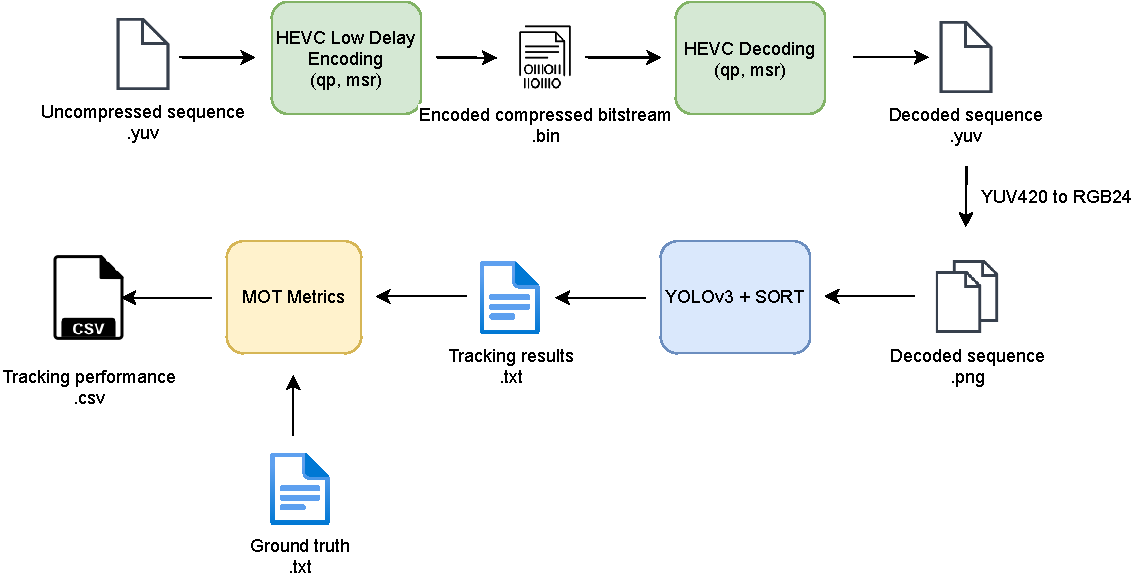
\includegraphics[width=1.0\linewidth]{img/experiment_pipeline.pdf}
  \caption[Pipeline for the experiment]
  {Pipeline for the experiment.}
  \label{fig:experiment_pipeline}
\end{figure}

